%!TEX program = xelatex
\documentclass[nobib, nohyper, a4paper, notoc, sfsidenotes,  twoside]{tufte-book}
% \XeTeXinputnormalization=1
\usepackage[ngerman]{babel}
\usepackage{fontspec}
\usepackage[babel,german=quotes]{csquotes}
\usepackage{polyglossia}
\usepackage[xetex,
            bookmarks=true,
            colorlinks=true,
            linktoc=section,
            pdfauthor={Your Name},
            pdftitle={The Title},
            pdfsubject={The Subject},
            pdfkeywords={Some Keywords},
            ]{hyperref}
\usepackage{booktabs}
\usepackage{svg}
\usepackage{amsmath}
\usepackage{xcolor,listings}
\colorlet{punct}{red!60!black}
\definecolor{background}{HTML}{EEEEEE}
\definecolor{delim}{RGB}{20,105,176}
\colorlet{numb}{magenta!60!black}
\lstset{ %
basicstyle=\normalfont\ttfamily,
numberstyle=\scriptsize,
stepnumber=1,
numbersep=8pt,
backgroundcolor=\color{background},
}

\lstdefinelanguage{json}{
    basicstyle=\normalfont\ttfamily,
    numberstyle=\scriptsize,
    stepnumber=1,
    numbersep=8pt,
    showstringspaces=false,
    breaklines=true,
    backgroundcolor=\color{background},
    literate=
     *{:}{{{\color{punct}{:}}}}{1}
      {,}{{{\color{punct}{,}}}}{1}
      {\{}{{{\color{delim}{\{}}}}{1}
      {\}}{{{\color{delim}{\}}}}}{1}
      {[}{{{\color{delim}{[}}}}{1}
      {]}{{{\color{delim}{]}}}}{1},
}
% tufte fix
\ifxetex
\newcommand{\textls}[2][5]{%
  \begingroup\addfontfeatures{LetterSpace=#1}#2\endgroup
}
\renewcommand{\allcapsspacing}[1]{\textls[15]{#1}}
\renewcommand{\smallcapsspacing}[1]{\textls[10]{#1}}
\renewcommand{\allcaps}[1]{\textls[15]{\MakeTextUppercase{#1}}}
\renewcommand{\smallcaps}[1]{\smallcapsspacing{\scshape\MakeTextLowercase{#1}}}
\renewcommand{\textsc}[1]{\smallcapsspacing{\textsmallcaps{#1}}}
\fi
% --
\makeatletter
\newcommand\chapterauthor[1]{}
\def\@chapterauthor{}
\fancypagestyle{mystyle}{%
\fancyhf{}%
\renewcommand{\chaptermark}[1]{\markboth{##1}{}}%
\fancyhead[LE]{\thepage\quad\smallcaps{\newlinetospace{\leftmark}}}% 
\fancyhead[RO]{\smallcaps{\newlinetospace{\@chapterauthor}}\quad\thepage}%
}
\makeatother


\usepackage{titlesec}
\titleformat{\chapter}% reformat chapter headings
     [hang]% like section, with number on same line
     {\huge}% formatting applied to whole
     {\thechapter}% Chapter number
     {0.5em}% space between # and title
     {}% formatting applied just to title

% Tufte parfill https://tex.stackexchange.com/questions/77999/remove-indent-of-paragraph-and-add-line-skip-with-tufte-latex
\makeatletter
% Paragraph indentation and separation for normal text
\renewcommand{\@tufte@reset@par}{%
  \setlength{\RaggedRightParindent}{0pt}%
  \setlength{\JustifyingParindent}{0pt}%
  \setlength{\parindent}{0pt}%
  \setlength{\parskip}{\baselineskip}%
}
\@tufte@reset@par

% Paragraph indentation and separation for marginal text
\renewcommand{\@tufte@margin@par}{%
  \setlength{\RaggedRightParindent}{0pt}%
  \setlength{\JustifyingParindent}{0pt}%
  \setlength{\parindent}{0pt}%
  \setlength{\parskip}{\baselineskip}%
}
\makeatother
\usepackage[export]{adjustbox}
\usepackage[caption=false]{subfig}

\usepackage{blindtext}

\usepackage{csvsimple}

\setdefaultlanguage[spelling=new,babelshorthands=true]{german}
\setotherlanguage[]{english}

\usepackage[parfill]{parskip}

% \setromanfont[Mapping=tex-text]{Linux Biolinum}
% \setsansfont[Mapping=tex-text]{Gill Sans}
\setmonofont[Mapping=tex-text,Scale=0.8]{Droid Sans Mono}
% \newfontfamily{\sym}{Font Awesome 5 Pro Regular}
% \newfontfamily{\sym}{Linux Biolinum}
% \newcommand*{\sym}{\fontfamily{FontAwesome}\selectfont}
\usepackage{scrextend}
\addtokomafont{labelinglabel}{\sffamily}

\usepackage{graphicx}
\usepackage[
    % sorting=nyt,
    isbn=false,
    style=authoryear-icomp,
    % citestyle=authoryear,
    % bibstyle=authoryear,
    % % natbib=true,
    % autocite=footnote,
    backend=biber,
    date=short
    ]{biblatex}
\addbibresource{bibliography/all.bib}



\usepackage{cleveref}
\captionsetup[subfigure]{subrefformat=simple,labelformat=simple}
\renewcommand\thesubfigure{(\alph{subfigure})}
% \usepackage{todonotes} % big performance impact


%layout
% \usepackage{showframe}
\usepackage{layouts}
\usepackage{epigraph}
% \setlength\epigraphwidth{5cm}
\setlength\epigraphrule{0pt}

\author{Jakob Schmolling}

% style settings

% numberings
\setcounter{secnumdepth}{1}
\setcounter{tocdepth}{1}

\definecolor{emph}{HTML}{5D5E5E}
\definecolor{alternative}{HTML}{083D77}
\definecolor{light}{HTML}{D0E1D4}
\definecolor{signal}{HTML}{F74511}
\definecolor{edge}{HTML}{0C120C}

% Macros
\newcommand{\sfigure}[2]{
    \begin{figure}
    \includegraphics[width=\textwidth]{#2} 
    \caption{#1}
    \end{figure}
}
\newcommand{\qq}[1]{
    \marginnote{{\color{signal}#1}}
}

\begin{document}
% \maketitle
\newcommand{\jc}[1]{\texttt{#1}}
\newsavebox{\titleimage}
%\savebox{\titleimage}{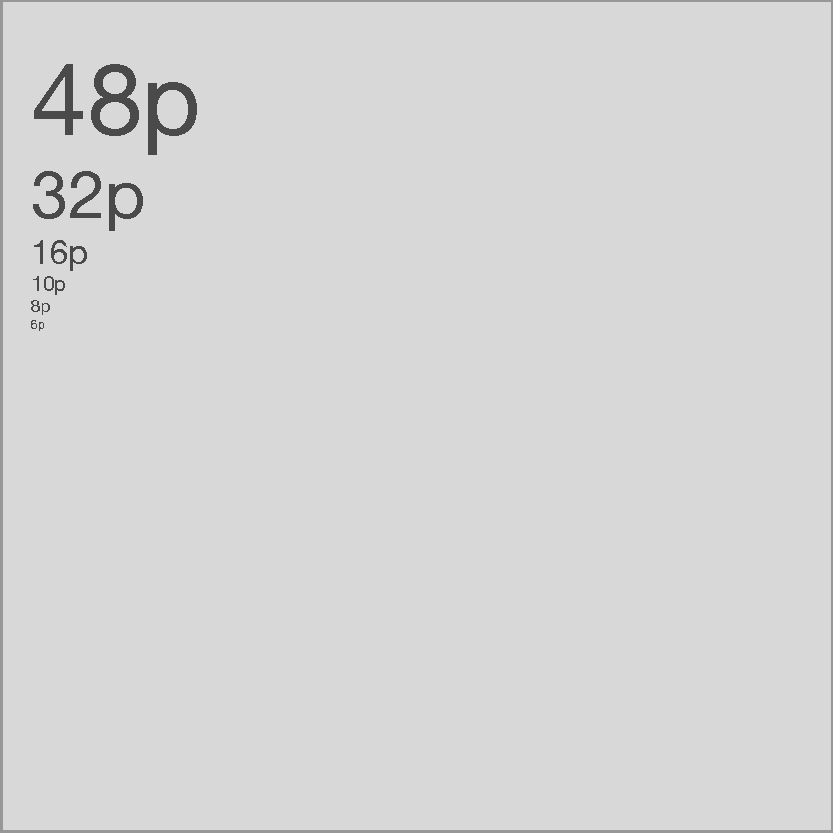
\includegraphics[width=12cm]{figures/font_sizes.pdf}}

\author{Jakob Schmolling}
\title[]{
\vfill
\usebox{\titleimage}\\
\noindent
\huge{Layout-Erkennung in digtalisierten Dokumenten mittels Neuronaler Netzwerke}\\
\noindent\Large{1.Korrektur}\\
% \noindent\Large{Untertitel der Arbeit}\\
% \noindent\Large{Untertitel der Arbeit}
}


\publisher[HTW Berlin]{HTW Berlin / \today}

\tableofcontents
\pagebreak
\chapter{Digtalisierten Dokumente}

% Warum scannt man Dokumente

% Was für Dokumente werden gescannt

% 
Schon in den 50er Jahren begann die Forschung im Bereich der Optischen Zeichenerkennung (engl. OCR)\autocite{BairdEvolutionDocumentImage2014}. OCR fand zuerst Anwendung in genau spezifizierten Problembereichen zum Beispiel die Erkennung von Druckbuchstaben einer Schreibmaschine. 
Je mehr Dokumente digitalisiert wurden, desto klare wurde es das Dokumente mehr als 
eine Kette von Zeichen sind. 

\section{Schritte in der Verarbeitung von Dokumentenbildern}
Dokumentensegmetierung
OCR
Klassifizierung siehe \cite{McConnaugheyLabeledSegmentationPrinted2017}
Flow
\section{Dokumentensegmetierung mittels CNN}
1. Ansatz von \autocite{ChenConvolutionalNeuralNetworks2017}
Superpixel segmentierung
Klassifizierung auf Superpixel statt Pixelebene.

2. Ansatz von \autocite{WickFullyConvolutionalNeural2017}

\section{SLIC Superpixel}
\cite{AchantaSLICSuperpixels2010}

\chapter{Selbstüberwachtes Lernen}

Jigsaw
\cite{NorooziUnsupervisedLearningVisual2016}
% \begin{figure}
%     \includegraphics[]{figures/graphs/exp.pdf} 
%     \caption{Image}
%   \end{figure}

\chapter{Umsetzung}

\section{Evaluierung}

\subsection{Metriken}
Die Evaluierung der Ergebnisse der Segmentierung erfolgt auf Pixelebene.
\cite{long_fully_2015} berechnet 4 Metriken.
Sei \(n_{ij}\) die Anzahl der Pixel der Klasse \(i\) die der Klasse \(j\) zugeordnet wurden.

% \csvautotabular{results/DIVA-HisDB.csv}

\newcommand{\resulttable}[2]{
    \begin{tabular}{l|r|r|r|r|r}%
        \hline
        \csvreader[head to column names, filter equal={\dataset}{#1}]{results/document_image_segmentation_results.csv}{}%
        {#2}
        \\\hline
        \end
        {tabular}
}

\resulttable{CB55}{\\ \name & \pixelacc & \FgPA & \meanacc & \meanIU & \fwIU}
\resulttable{CSG18}{\\  \pixelacc & \FgPA & \meanacc & \meanIU & \fwIU}
\resulttable{CSG863}{\\  \pixelacc & \FgPA & \meanacc & \meanIU & \fwIU}



\printbibliography[heading=bibintoc, title={Literaturverzeichnis}]\clearpage
% \printbibliography[heading=bibintoc, keyword={online}, title={Onlinequellen}]\clearpage
% \printbibliography[heading=bibintoc, keyword={image}, title={Bildquellen}]\clearpage

\pagebreak
\section*{Eidesstattliche Erklärung}
Hiermit versichere ich, dass ich die vorliegende Arbeit selbstständig verfasst und keine ande- ren als die angegebenen Hilfsmittel benutzt habe. Alle aus fremden Quellen im Wortlaut oder dem Sinn nach entnommenen Aussagen sind durch Angaben der Herkunft kenntlich gemacht.
Die Arbeit wurde bisher in gleicher oder ähnlicher Form keiner anderen Prüfungskommissi- on vorgelegt und auch nicht veröffentlicht.

\vspace{3cm}
\parbox{4cm}{\centering \hrule\strut \centering\footnotesize Ort, Datum} 
\hfill
\parbox{4cm}{\hrule\strut \centering\footnotesize Unterzeichner}

\end{document}